\section{Kovarians test} \label{subsec:kovarians_test}
I dette afsnit introduceres en test, der kan tildele \(p\)-værdier til prædiktorerne, som er udvalgt af lasso.
Testen er baseret på LARS algoritmen og blev introduceret i \citep{lockhart}.

Betragt det velkendte lineære regressionssetup
\begin{align}
\y = \X \tbeta + \boldsymbol{\epsilon}, \quad \boldsymbol{\epsilon} \sim N\del{\mathbf{0}, \sigma^2 \mathbf{I}_n}, \label{eq:set-up}
\end{align}
hvor \(\y\) er en \(n \times 1\) vektor med responsvariablen, \(\X\) er en \(n \times p\) matrix med prædiktorer og \(\tbeta\) er en \(p \times 1\) vektor, som skal estimeres.

Vi antager, at søjlerne i \(\X\) er i generel position, for at sikre at løsningsstien for LARS algoritmen med lasso modifikationen er entydig (se definition \ref{defn:general_position}).
Vi ønsker, at teste om prædiktoren, som tilføjes til den aktive mængde i step \(k\), er signifikant.
Den aktive mængde betegner somsagt prædiktorerne med ikke-nul koefficienter, og igen lader vi \(\lambda_k\) betegne \(k\)'te step i løsningsstien.
Lad \(\A_{k-1}\) betegne den aktive mængde i step \(k-1\) inden prædiktoren tilføjes, og lad \(\tilde{\tbeta}^\text{lasso}_{\A_{k-1}} \del{\lambda_{k+1}}\) være løsningen i \(\lambda_{k+1}\) ved kun at anvende prædiktorerne i \(\A_{k-1}\).
Denne løsning er eksplicit givet ved 
\begin{align*}
\tilde{\tbeta}^\text{lasso}_{\A_{k-1}} \del{\lambda_{k+1}} = \argmin_{\tbeta_{\A_{k-1}} \in \R^{\vert \A_{k-1} \vert}} \cbr{ \left\Vert \y - \X_{\A_{k-1}} \tbeta_{\A_{k-1}} \right\Vert_2^2 + \lambda_{k+1} \left\Vert \tbeta_{\A_{k-1}} \right\Vert_1},
\end{align*}
hvor \(\X_{\A_{k-1}}\) er en matrix, der består af søjlerne i \(\X\), som svarer til prædiktorerne i \(\A_{k-1}\).
Lad \(\widehat{\tbeta}^\text{lasso} \del{\lambda_{k+1}}\) betegne løsningen i \(\lambda_{k+1}\) udfra prædiktorerne \(\A_{k-1} \cup \cbr{j}\).
Da kan vi definere teststørrelsen af kovarians testen
\begin{align}
T_k^\text{cov} = \frac{1}{\sigma^2} \del{ \left\langle \y, \X \widehat{\tbeta}^\text{lasso} \del{\lambda_{k+1}} \right\rangle - \left\langle  \y, \X_{\A_{k-1}} \tilde{\tbeta}^\text{lasso}_{\mathcal{A}_{k-1}} \del{\lambda_{k+1}} \right\rangle}. \label{eq:6.5}
\end{align}
Intuitivt er teststørrelsen af kovarians testen i \eqref{eq:6.5} en funktion af differensen mellem \(\X \widehat{\tbeta}^\text{lasso}\) og \(\X_{\A_{k-1}} \tilde{\tbeta}^\text{lasso}_{\A_{k-1}}\), dvs de fittede værdier givet ved at inkludere og undlade \(j\)'te prædiktor i den nuværende aktive mængde.
Navnet af testen kommer af, at tælleren i \eqref{eq:6.5} kan betragtes som differensen mellem empiriske (ikke-centreret) kovarianser og et lille led. 
\footnote{Lad \(\y = \y - \tmu + \tmu\) med \(\tmu = \X \tbeta^*\), da kan tælleren af \eqref{eq:6.5} omskrives \(T_k^\text{cov} = \left\langle \y - \tmu, \X \widehat{\tbeta}^\text{lasso} \del{\lambda_{k+1}} \right\rangle - \left\langle \y - \tmu, \X_{\A_{k-1}} \tilde{\tbeta}^\text{lasso}_{\A_{k-1}} \del{\lambda_{k+1}} \right\rangle + \left\langle \tmu, \X \widehat{\tbeta}^\text{lasso} \del{\lambda_{k+1}} - \X_{\A_{k-1}} \tilde{\tbeta}^\text{lasso}_{\A_{k-1}} \del{\lambda_{k+1}} \right\rangle\).
De første to led er empiriske kovarianser og det sidste led er typisk lille.}
Desto større kovarians af \(\y\) og \(\X \widehat{\tbeta}^\text{lasso}\) sammenlignet med \(\X_{\A_{k-1}} \tilde{\tbeta}^\text{lasso}_{\A_{k-1}}\), desto vigtigere er \(j\)'te prædiktor i modellen \(\A_{k-1} \cup \cbr{j}\).
%Kovarians teststørrelsen evalueres i næste knot \(\lambda_{k+1}\), da \(j\)'te koefficient stadig er lig nul i \(\lambda_k\).
%I \(\lambda = \lambda_{k+1}\), ses den ...
% og dermed
%\begin{align*}
%\X \hat{\beta} \del{\lambda_k} = \X_{\A_{k-1}} \hat{\beta}_{\A_{k-1}} \del{\lambda_k} = \X_{\A_{k-1}} \tilde{\beta}_{\A_{k-1}} \del{\lambda_k}
%\end{align*}
%Det naturlig valg for tuning parameteren i \eqref{eq:6.5} er derfor \(\lambda= \lambda_{k+1}\).

Under nulhypotesen at lasso modellen med den aktive mængde \(\A_{k-1}\) indeholder alle sande aktive variable, dvs \(\hyp_0: \mathcal{A}_{k-1} \supseteq \text{supp} \del{\tbeta^*}\) (se definition \ref{defn:supp}), hvor \(\tbeta^*\) er den sande koefficientvektor, da har teststørrelsen i \eqref{eq:6.5} en asymptotisk standard eksponentiel fordeling
\begin{align*}
T_k^\text{cov} \overset{d}{\rightarrow} \text{Exp}\del{1}.
\end{align*}
Vi henviser til s. 425-441 i \citep{lockhart}, hvor resultatet bevises. 
Hvis \(\sigma^2\) er ukendt, kan den estimeres under den fulde model \(\widehat{\sigma}^2 = \frac{1}{n-p} \text{SSR}_p\). 
Dette indsættes i \eqref{eq:6.5}, og eksponential testen bliver en eksakt \(F_{2,n-p}\) test. \\[2mm]

\begin{eks}
For diabetes data ønsker vi at udregne \(p\)-værdien for prædiktoren \texttt{hdl}, som tilføjes til den aktive mængde i fjerde step af LARS algoritmen (se figur \ref{fig:diabetes_covTest}). 
Da skal vi udregne kovariansen i \(\lambda_5\), der er givet ved \(\left\langle \y, \X \widehat{\tbeta}^\text{lasso} \del{\lambda_5} \right\rangle\).
Herefter fjernes prædiktoren \texttt{hdl}, hvilket giver den aktive mængde \(\A_{3}\), vi refitter i \(\lambda_5\) og udregner igen kovariansen i \(\lambda_5\), der er givet ved \(\left\langle  \y, \X_{\A_{3}} \tilde{\tbeta}^\text{lasso}_{\mathcal{A}_{3}} \del{\lambda_{5}} \right\rangle\).
Teststørrelsen af kovarians testen er da givet ved
\begin{align*}
T_4^\text{cov} = \frac{1}{\sigma^2} \del{ \left\langle \y, \X \widehat{\tbeta}^\text{lasso} \del{\lambda_{5}} \right\rangle - \left\langle  \y, \X_{\A_{3}} \tilde{\tbeta}^\text{lasso}_{\mathcal{A}_{3}} \del{\lambda_{5}} \right\rangle}.
\end{align*}
%
\begin{figure}[H]
\centering
\scalebox{0.6}{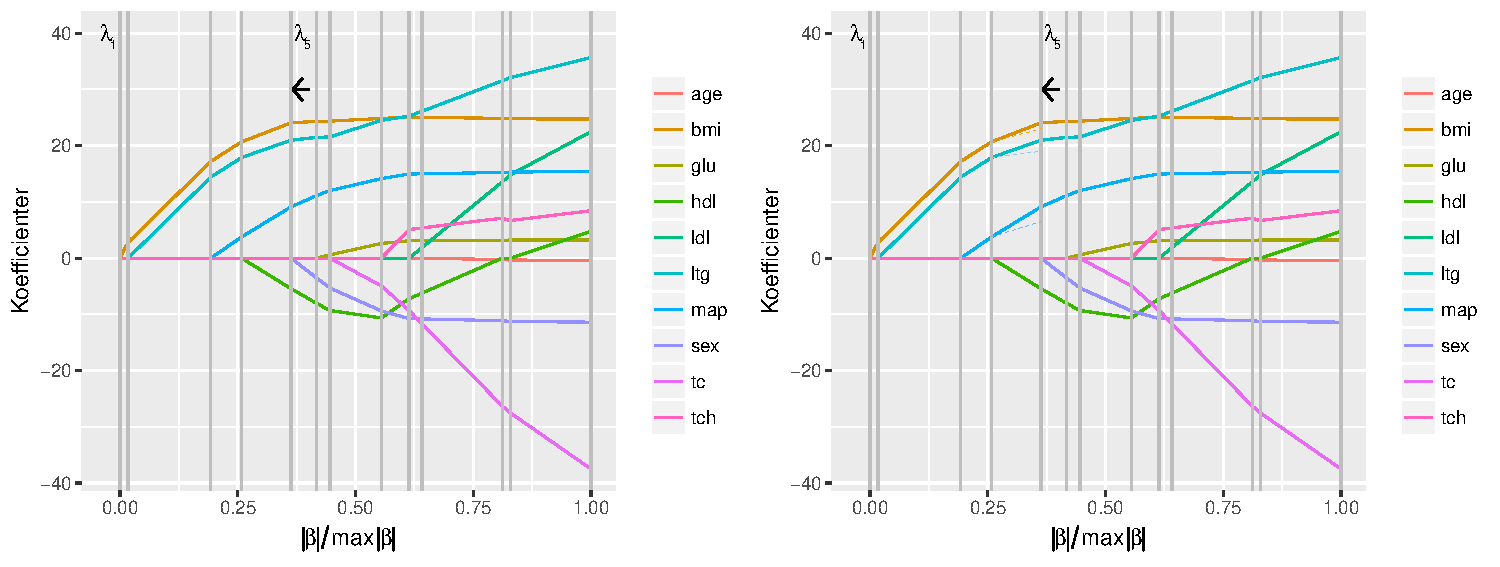
\includegraphics{fig/img/diabetes_covTest.pdf}}
\caption{Illustration af kovarians testen for prædiktoren \texttt{hdl}.} \label{fig:diabetes_covTest}
\end{figure}
%
Resultatet af kovarians testen anvendt på diabetes data er givet i tabel \ref{tab:diabetes_covTest}.
Nulhypotesen afvises for \texttt{bmi}, \texttt{ltg}, \texttt{map} og \texttt{hdl}, som tilføjes til den aktive mængde i step 1-4, hvilket betyder, at disse prædiktorer er signifikante.
For de resterende prædiktorer kan nulhypotesen ikke afvises.
%
\begin{table}[ht] 
\centering 
\begin{tabular}{lccc}
%\multicolumn{3}{l}{LARS algoritmen med lasso modifikation} \\
\toprule
Prædiktor & Cov test & \(p\)-værdi \\
\midrule
\texttt{bmi} & 9.0612 & 0.0000 \\
\texttt{ltg} &50.9187 & 0.0000 \\
 \texttt{map}     &       5.5886 & 0.0040 \\
 \texttt{hdl}      &    5.9933 & 0.0027 \\
\texttt{sex}     &   4.8039 & 0.0086 \\
\texttt{glu}     &  0.1593 & 0.8528 \\
\texttt{tc}  &         3.2848 & 0.0384 \\
\texttt{tch}    &        0.6153 & 0.5409 \\
\texttt{ltg}    &        0.1639 & 0.8489 \\
\texttt{age} &       0.0150 & 0.9851 \\ \bottomrule
\end{tabular}
\caption{Kovarians testen for LARS algoritmen med lasso modifikation for diabetes data. Vi har, at \(\widehat{\sigma}^2 = 54.0975\) og nulfordelingen \(F_{2,432}\).} \label{tab:diabetes_covTest}
\end{table} 
\end{eks}

Kovarians testen er det naturlige analog til resultaterne for frihedsgrader for lasso og LARS.
Som nævnt tidligere har lasso med \(k\) ikke-nul koefficienter \(k\) frihedsgrader, mens LARS anvender en frihedsgrad for hvert step.
Kovarians testen har middelværdi lig en, som er antallet af frihedsgrader per step.
Hermed kan man sige at Exp\(\del{1}\) fordelingen svarer til \(\chi_1^2\) fordelingen for adaptive procedurer.

%Kovarians testen har nogle begrænsninger.
%Først skal der gælde, at kolonner af \(\X\) er i generel position.
%%Hvis der eksisterer en kategorisk variabel blandt prædiktorerne, og den resulterende variabel beskrives af dummy variable, da er antagelse om at kolonnerne af \(\X\) er i general position altså ikke overholdt.
%Derudover tager testen ikke højde for, hvis nogle variable medtages i modellen mere end én gang (som er tilladt for lasso modifikationen af LARS algoritmen), da behandles hver situation separat og testene udføres separat.
%Til sidst er testen kun asymptotisk.
%
%I næste afsnit introduceres en test som kan anvendes efter modeludvælgelse og som giver en eksakt fordeling af teststørrelsen.